% Canonical extraction of the existing L3 row/column/subgrid drawing.
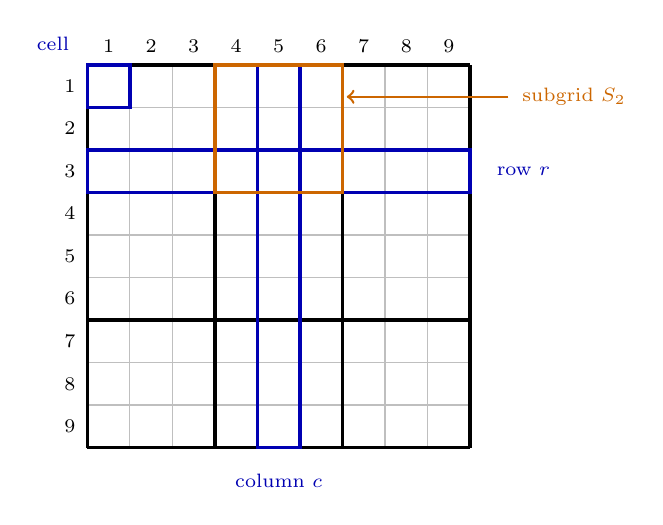
\begin{tikzpicture}[x=0.54cm,y=0.54cm]
  \foreach \i in {0,...,9} {
    \draw[gray!50, line width=0.4pt] (\i,0) -- (\i,9);
    \draw[gray!50, line width=0.4pt] (0,\i) -- (9,\i);
  }
  \foreach \i in {0,3,6,9} {
    \draw[black, line width=1.2pt] (\i,0) -- (\i,9);
    \draw[black, line width=1.2pt] (0,\i) -- (9,\i);
  }
  \foreach \i [evaluate=\i as \pos using \i-0.5] in {1,...,9} {
    \node[font=\scriptsize, anchor=south] at (\pos,9.05) {\i};
    \node[font=\scriptsize, anchor=east] at (-0.05,9-\pos) {\i};
  }
  % highlight one cell, one row, one column, one subgrid
  \draw[blue!70!black, line width=1.2pt] (0,8) rectangle (1,9);
  \node[blue!70!black, anchor=east, font=\scriptsize] at (-0.2,9.5) {cell};
  \draw[blue!70!black, line width=1.2pt] (0,6) rectangle (9,7);
  \node[blue!70!black, anchor=west, font=\scriptsize] at (9.4,6.5) {row $r$};
  \draw[blue!70!black, line width=1.2pt] (4,0) rectangle (5,9);
  \node[blue!70!black, anchor=north, font=\scriptsize] at (4.5,-0.4) {column $c$};
  \draw[orange!80!black, line width=1.4pt] (3,6) rectangle (6,9);
  \draw[orange!80!black, ->, line width=0.9pt] (9.9,8.25) -- (6.1,8.25);
  \node[orange!80!black, anchor=west, font=\scriptsize] at (10.0,8.25)
    {subgrid $S_2$};
\end{tikzpicture}
